\documentclass{report}

% Language setting
\usepackage[main=portuguese, english]{babel}
\usepackage{csquotes}

% Set page size and margins
\usepackage[a4paper,top=2cm,bottom=2cm,left=3cm,right=3cm,marginparwidth=1.5cm]{geometry}

% Useful packages
\usepackage{ulem}
\usepackage{parskip}
\usepackage{indentfirst}
\usepackage{setspace}
\usepackage{amsmath}
\usepackage{array}

\usepackage{graphicx}
\usepackage{xcolor}
\usepackage{colortbl}
\usepackage{subfigure}
\usepackage{titlesec}
\usepackage[colorlinks=false, allbordercolors={0 0 0}, pdfborderstyle={/S/U/W 0.25}]{hyperref}
\usepackage[hypcap=true]{caption}
\usepackage{enumitem}
\usepackage{outlines}
\usepackage{soul}
\usepackage{ragged2e}

% Set section numbering from 1.1
\renewcommand{\thesection}{\arabic{section}.1}
\newcolumntype{P}[1]{>{\centering\arraybackslash}p{#1}}
\newcolumntype{M}[1]{>{\centering\arraybackslash}m{#1}}

\let\oldsection\section
\renewcommand\section{\clearpage\oldsection}

% Change section formatting
\titleformat{\section}
  {\fontsize{12}{15}\selectfont\bfseries}{\thesection}{1em}{}

% Configure indentations
\setlength{\parindent}{1.5cm}

\begin{document}

    \begin{titlepage}
        \centering
        
        \LARGE {Universidade Federal do Rio Grande do Sul \\ Instituto de Informática}
    
        \begin{figure}[h!]
            \centering
            \subfigure
            {
\includegraphics[width=0.35\linewidth]{images/logos/UFRGS.png}}
            \hspace{1cm}
            \subfigure
            {
\includegraphics[width=0.35\linewidth]{images/logos/INF.png}}
        \end{figure}
    
        \LARGE {INF01113 \\ Organização de Computadores B}
        
        \vfill
        {\noindent\hrulefill \\
        \bfseries \Huge{Trabalho Prático 1 - Tarefa 09} \\ \LARGE{Implementação de Instruções no MIPS} \\
        \noindent\hrulefill}
        
        \vfill
        {\LARGE Bruno Alexandre Hofstetter Bourscheid (00550177) \\ Fernando Longhi de Andrade (00580366) \\ Luiz Augusto Ponzoni Schmidt (00580108) \\ Miguel Dutra Fontes Guerra (00342573) \\ Pedro Lubaszewski Lima (00341810) \\~\\ Turma B}
    
        \vfill
        {\LARGE 19 de abril de 2025}
        
    \end{titlepage}

    \renewcommand{\contentsname}{Sumário}
    \tableofcontents
    \clearpage
    \addtocontents{toc}{\protect\thispagestyle{empty}}

    \section{MIPS Singlecycle}
        \subsection{Modificações no Bloco Operativo}
        Para começar, segue uma ilustração de como estava inicialmente a parte operativa do MIPS Singleclycle:
        \begin{figure}[h!]
            \centering
            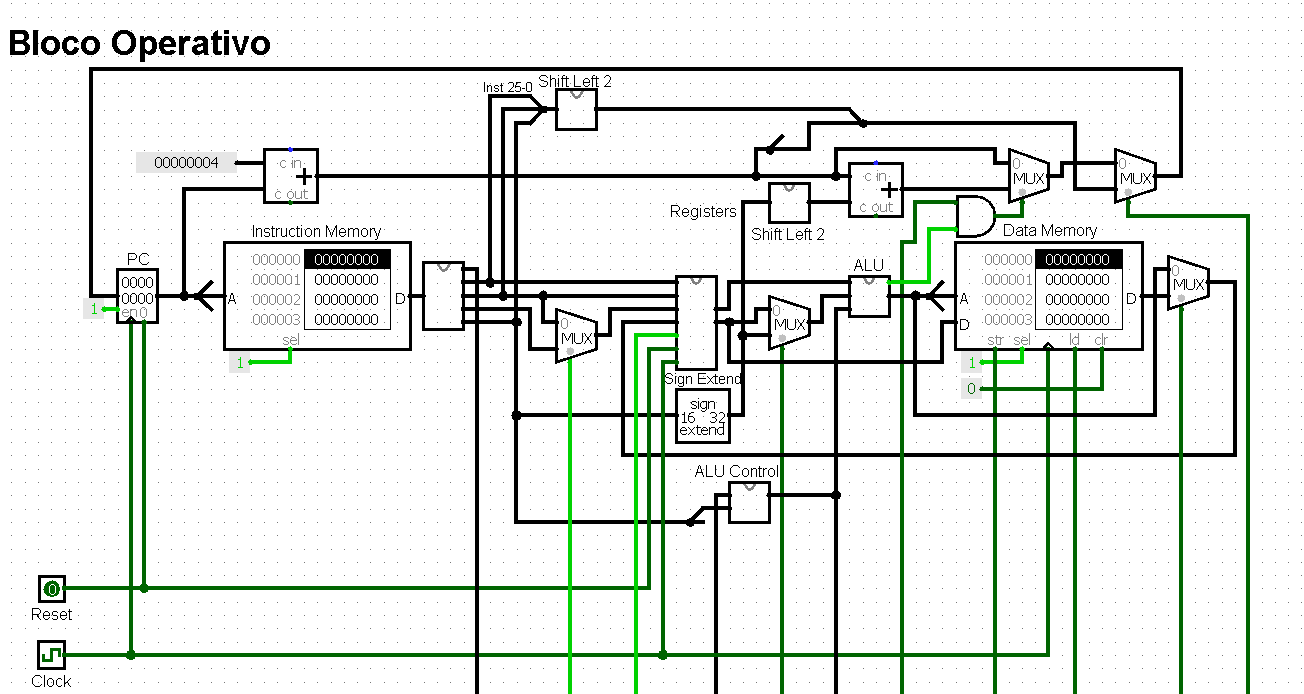
\includegraphics[width=\linewidth]{images/prints/Monocycle/Bloco Operativo Monocycle Antes.png}
            \caption{\label{print:singlecycle_ob_before} MIPS Singlecycle - Bloco Operativo Antes}
        \end{figure}

        Essa parte operativa foi modificada de acordo com as instruções adicionadas ao MIPS Singlecycle:
        \begin{itemize}
            \item Adicionada operação multiplicação na ALU;
            \item Adicionada saída dos bits superiores da multiplicação na ALU;
            \item Adicionada saída IsMULT da ALU;
            \item Adicionados registradores especiais LO e HI;
            \item Atualizada a flag 0 na ALU;
            \item Adicionado comparador para BLTZ e SLTIU;
            \item Adicionado sign extend para o BLTZ e SLTIU;
            \item Adicionado splitter para LB;
            \item Adicionado sign extend para LB;
            \item Atualizado o splitter para a Data Memory.
        \end{itemize}

        \clearpage
        Segue uma ilustração de como ficou a parte operativa do MIPS Singlecycle após as modificações acima listadas:
        \begin{figure}[h!]
            \centering
            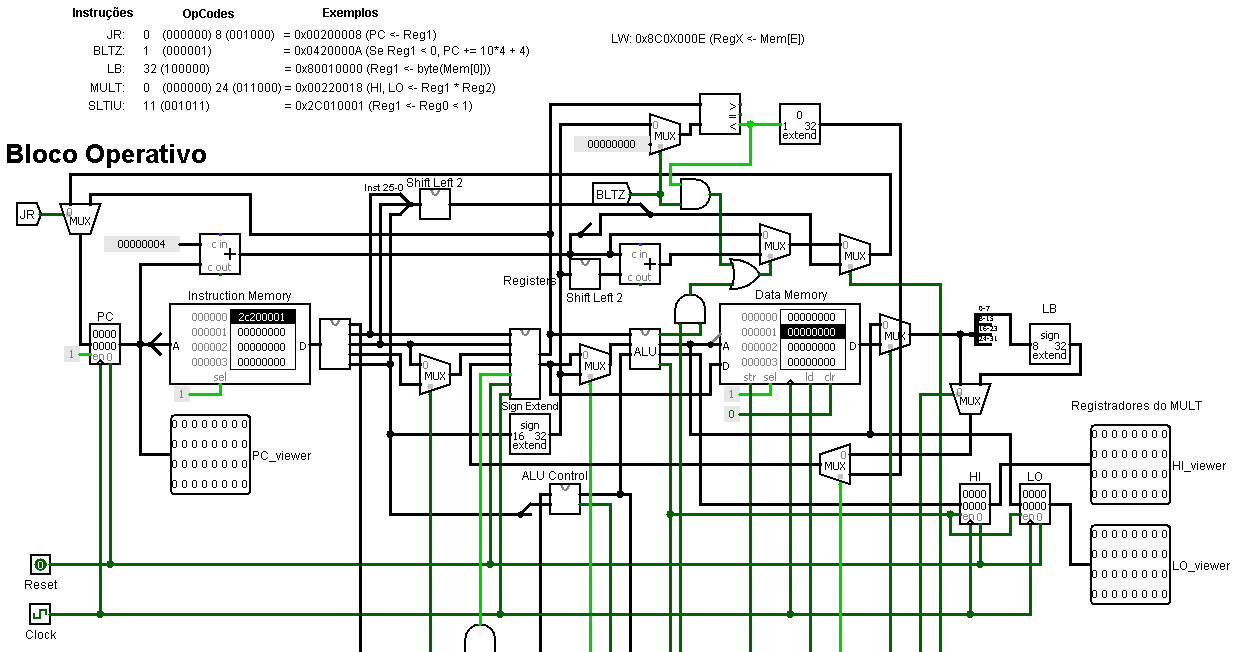
\includegraphics[width=\linewidth]{images/prints/Monocycle/Bloco Operativo Monocycle Depois.png}
            \caption{\label{print:singlecycle_ob_after} MIPS Singlecycle - Bloco Operativo Depois}
        \end{figure}

        \subsection{Modificações no Bloco de Controle}
        Já para a parte de controle, segue uma representação inicial do MIPS Singlecycle:
        \begin{figure}[h!]
            \centering
            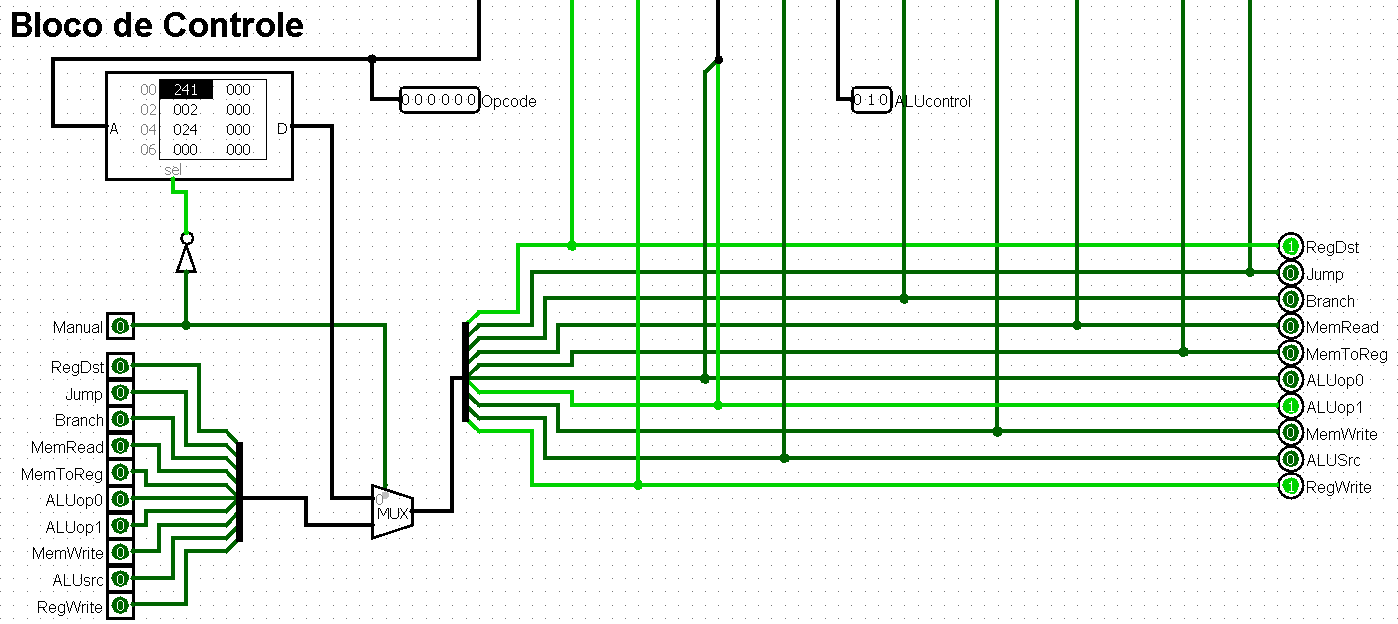
\includegraphics[width=\linewidth]{images/prints/Monocycle/Bloco de Controle Monocycle Antes.png}
            \caption{\label{print:singlecycle_cb_before} MIPS Singlecycle - Bloco Controle Antes}
        \end{figure}

        Com ela em mente, foram feitas as seguintes modificações:
        \begin{itemize}
            \item Criados os sinais de controle LB, SLTIU, BLTZ, JR e IsMult;
            \item Atualizado o ALU Control para as instruções de MULT e JR;
            \item Adicionado MUX para o BLTZ;
            \item Adicionado controle de branch para BLTZ;
            \item Adicionado controle de RegWrite usando IsMULT;
            \item Adicionado MUX para o JR;
            \item Adicionado MUX para LB;
            \item Adicionado MUX para SLTIU.
        \end{itemize}

        Abaixo segue também a codificação em memória ROM de controle das novas instruções:
        \begin{itemize}
            \item ROM para JR: 0x0241 end 0x00;
            \item ROM para BLTZ: 0x0404 end 0x01;
            \item ROM para LB: 0x0B18 end 0x20;
            \item ROM para MULT: 0x0241 end 0x00;
            \item ROM para SLTIU: 0x1300 end 0x0B.
        \end{itemize}

        Dessa forma, a parte de controle do processador terminou da seguinte forma:
        \begin{figure}[h!]
            \centering
            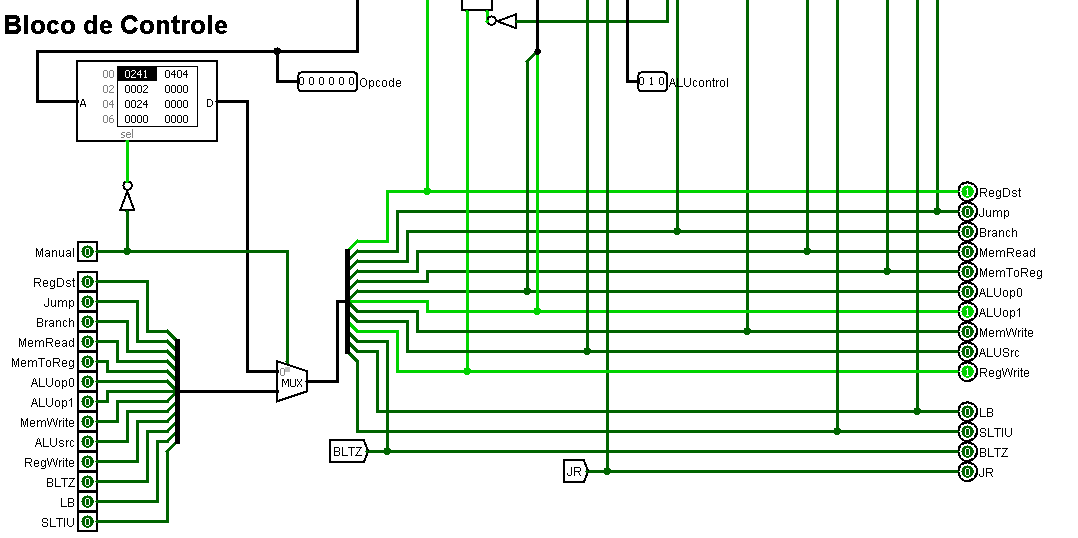
\includegraphics[width=\linewidth]{images/prints/Monocycle/Bloco de Controle Monocycle Depois.png}
            \caption{\label{print:singlecycle_cb_after} MIPS Singlecycle - Bloco Controle Depois}
        \end{figure}

        Algumas dessas modificações aqui listadas foram mostradas em mais detalhes na subseção anterior.

        \clearpage
        \subsection{Testes de Implementação}

        Para comprovar que essas mudanças acima trouxeram a correta implementação das instruções especificados neste trabalho,
        abaixo seguem os testes realizados com imagens e a respectiva sequência de instruções:
        
        \begin{itemize}
            \item Teste da Instrução JR:
                \subitem JR: PC $\leftarrow$ Reg1
                \subitem 0x8C010000; Reg1 $\leftarrow$ Mem[0] (3)
                \subitem 0x00200008; PC $\leftarrow$ Reg1 (3)
        \end{itemize}

        \begin{figure}[h!]
            \centering
            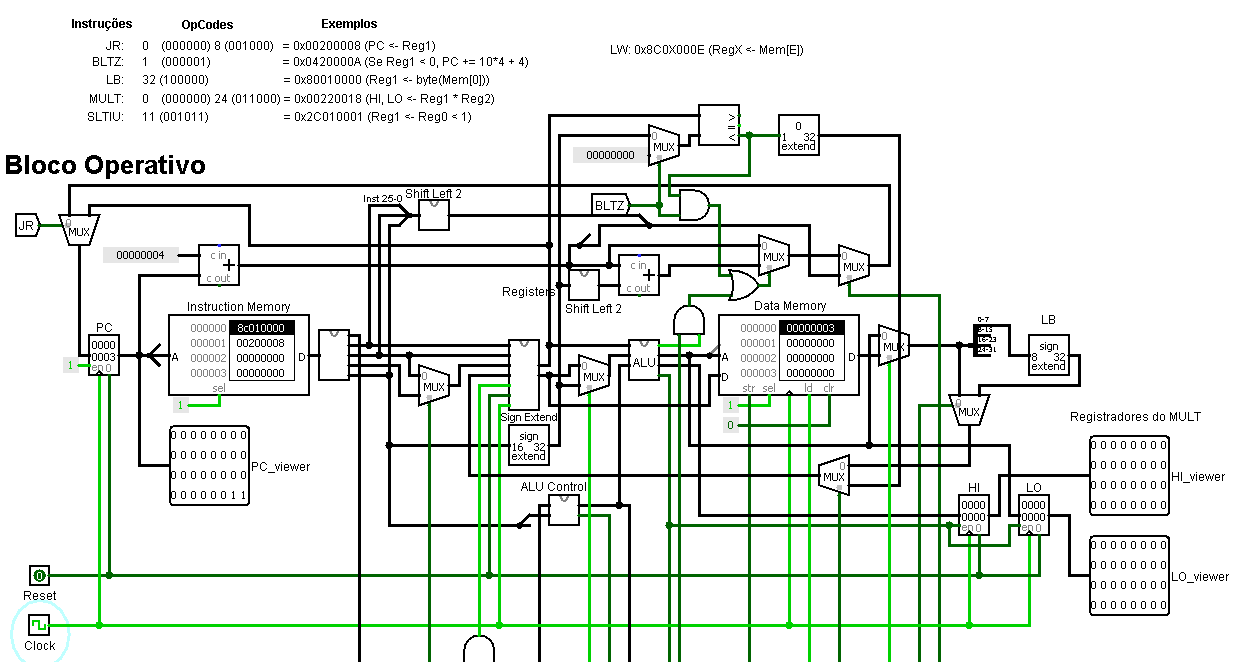
\includegraphics[width=\linewidth]{images/prints/Monocycle/Teste JR.png}
            \caption{\label{print:singlecycle_test_JR} MIPS Singlecycle - Teste JR}
        \end{figure}

        \begin{itemize}
            \item Teste da Instrução BLTZ:
                \subitem BLTZ: if Reg1 $<$ 0 then PC += IMED$\cdot$4 + 4 (IMED = 10)
                \subitem 0x8C010000; Reg1 $\leftarrow$ Mem[0] (-1 (0xFFFFFFFF))
                \subitem 0x0420000A; PC += IMED$\cdot$4 + 4 (PC = 48)
        \end{itemize}

        \begin{figure}[h!]
            \centering
            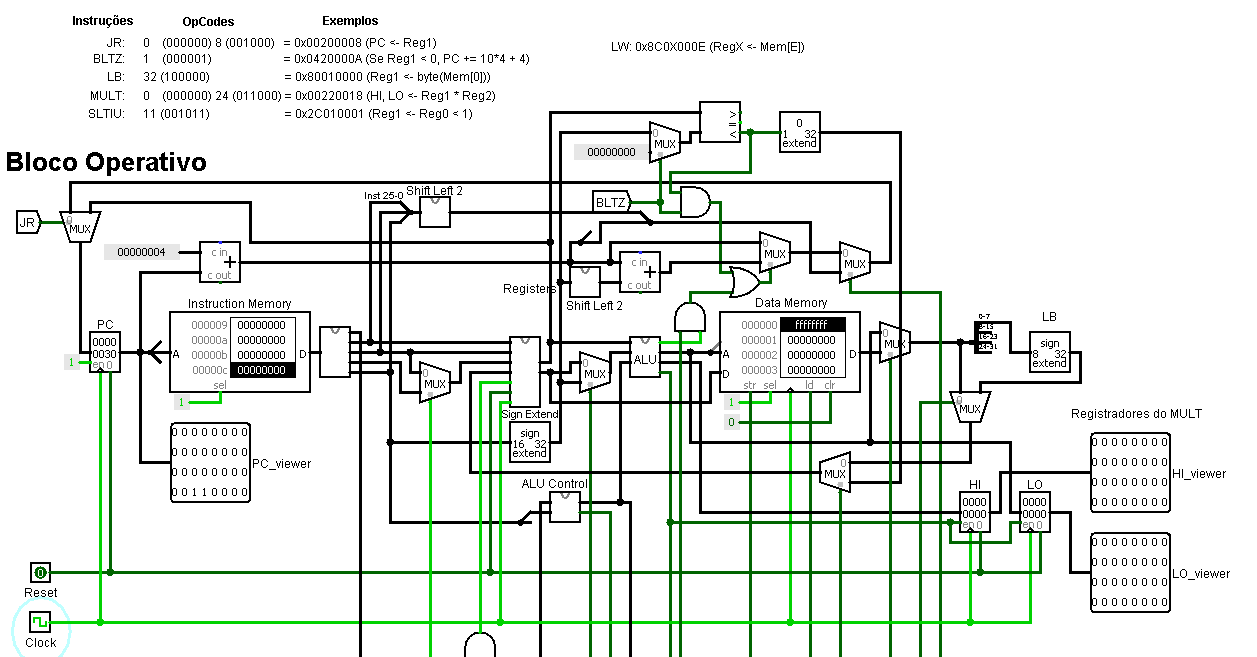
\includegraphics[width=\linewidth]{images/prints/Monocycle/Teste BLTZ.png}
            \caption{\label{print:singlecycle_test_BLTZ} MIPS Singlecycle - Teste BLTZ}
        \end{figure}

        \begin{itemize}
            \item Teste da Instrução LB:
                \subitem LB: Reg1 $\leftarrow$ byte(Mem[0]) (3)
                \subitem 0x80010000; Reg1 $\leftarrow$ byte(Mem[0])
        \end{itemize}

        \begin{figure}[h!]
            \centering
            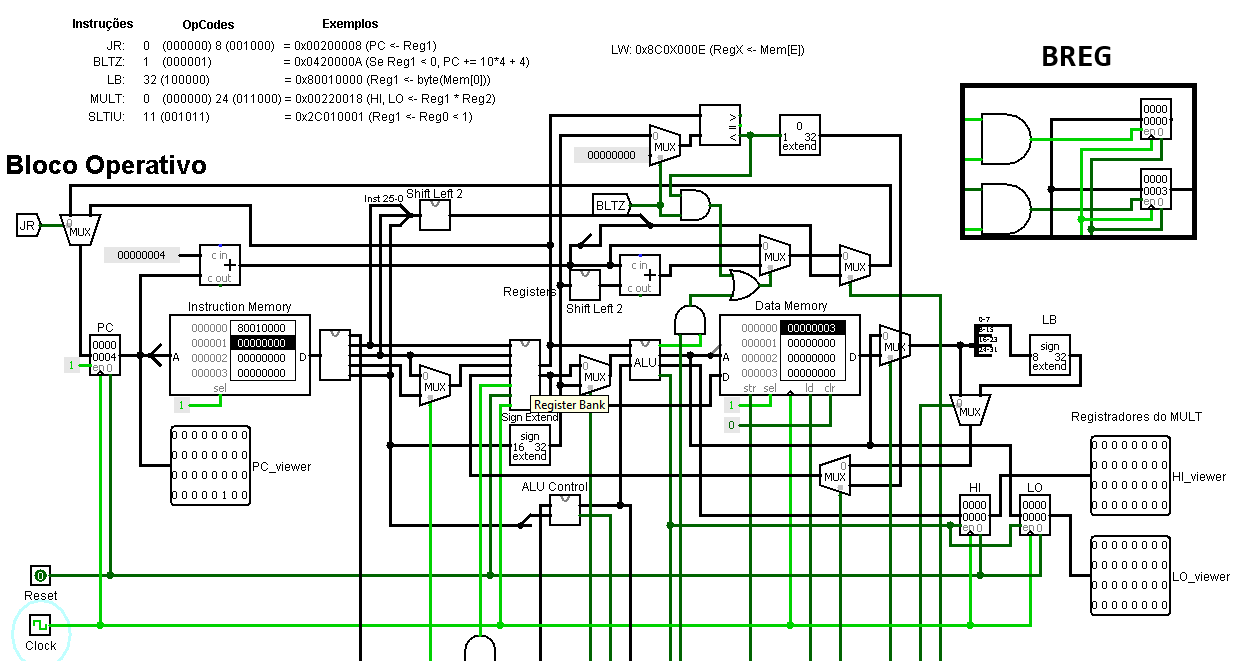
\includegraphics[width=\linewidth]{images/prints/Monocycle/Teste LB.png}
            \caption{\label{print:singlecycle_test_LB} MIPS Singlecycle - Teste LB}
        \end{figure}

        \begin{itemize}
            \item Teste da Instrução MULT:
                \subitem MULT: HI, LO $\leftarrow$ Reg1 $\cdot$ Reg2
                \subitem 0x8C010000; Reg1 $\leftarrow$ Mem[0] (3)
                \subitem 0x8C020001; Reg2 $\leftarrow$ Mem[1] (4)
                \subitem 0x00220018; HI, LO $\leftarrow$ Reg1 $\cdot$ Reg2 (HI = 0, LO = 12)
        \end{itemize}

        \begin{figure}[h!]
            \centering
            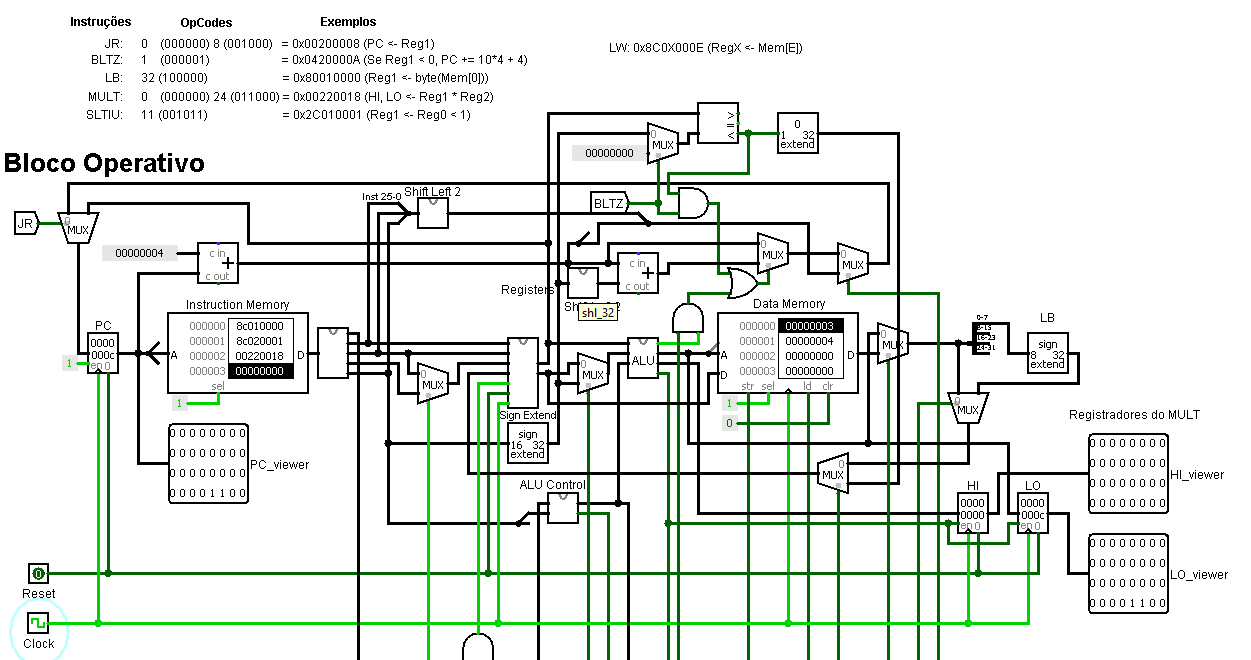
\includegraphics[width=\linewidth]{images/prints/Monocycle/Teste MULT.png}
            \caption{\label{print:singlecycle_test_MULT} MIPS Singlecycle - Teste MULT}
        \end{figure}

        \clearpage
        \begin{itemize}
            \item Teste da Instrução SLTIU:
                \subitem SLTIU: Reg1 $\leftarrow$ Reg0 $<$ IMED (1)
                \subitem 0x2C010001; Reg1 $\leftarrow$ Reg0 $<$ 1 (Reg1 = 1)
        \end{itemize}

        \begin{figure}[h!]
            \centering
            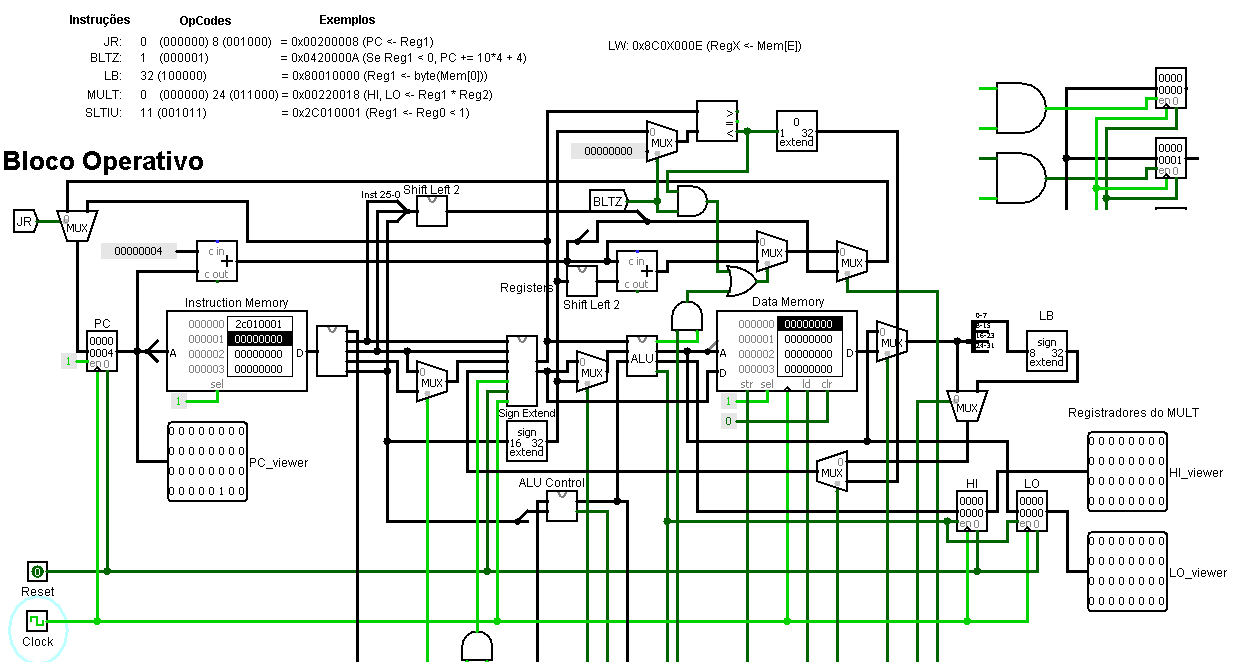
\includegraphics[width=\linewidth]{images/prints/Monocycle/Teste SLTIU.png}
            \caption{\label{print:singlecycle_test_SLTIU} MIPS Singlecycle - Teste SLTIU}
        \end{figure}

    \section{MIPS Multicycle}
        \subsection{Modificações no Bloco Operativo}

        \subsection{Modificações no Bloco de Controle}
        Além da adição de dois sinais (isBLTZ/isSLTIU)Foram modificadas as ROMs de controle de NextState e Saída, na primeira as alterações se deram pelas implementações da lógica de estado para as novas instruções de OPCode()
        
        \subsection{Estados de Controle}
        São utilizados no projeto 12 estados diferentes, contendo instruções de 3 a 5 ciclos, todas representadas na FSM anexada a seguir:
        \begin{figure}[h!]
            \centering
            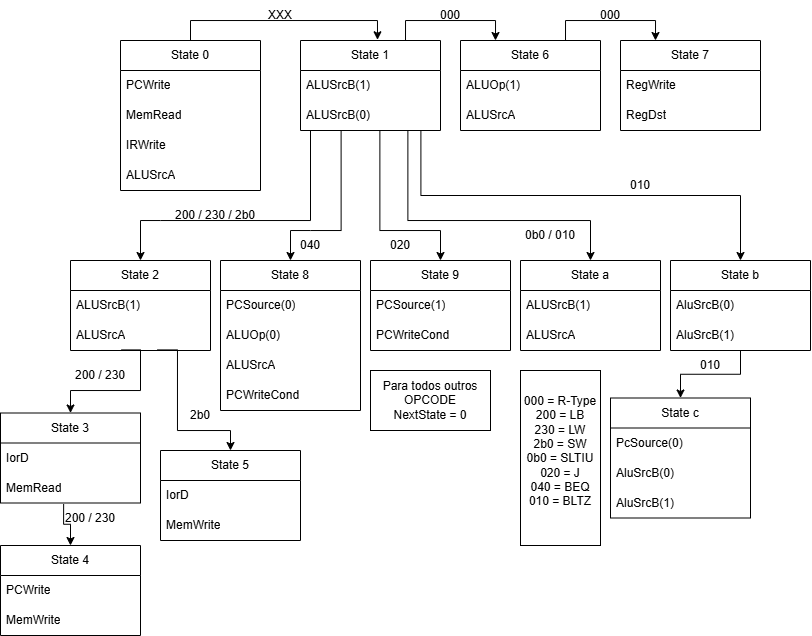
\includegraphics[width=\linewidth]{images/prints/Multicycle/FSM Multicycle.png}
            \caption{\label{print:FSM_Multicycle} MIPS Multicycle - Maquina de estados Multicycle}
        \end{figure}
        Nota-se que os nodos representam os estados de controle, enquanto as arestas os OPCodes, assim formando uma máquina de Moore com as saídas em "1" de cada estado notadas em cada nodo.

        \subsection{Testes de Implementação}

    \section{MIPS Pipeline}
        \subsection{Modificações no Bloco Operativo}
        Primeiramente, segue uma visão de como estava a implementação do MIPS com pipeline antes
        do acrescimo das novas instruções:
        \begin{figure}[h!]
            \centering
            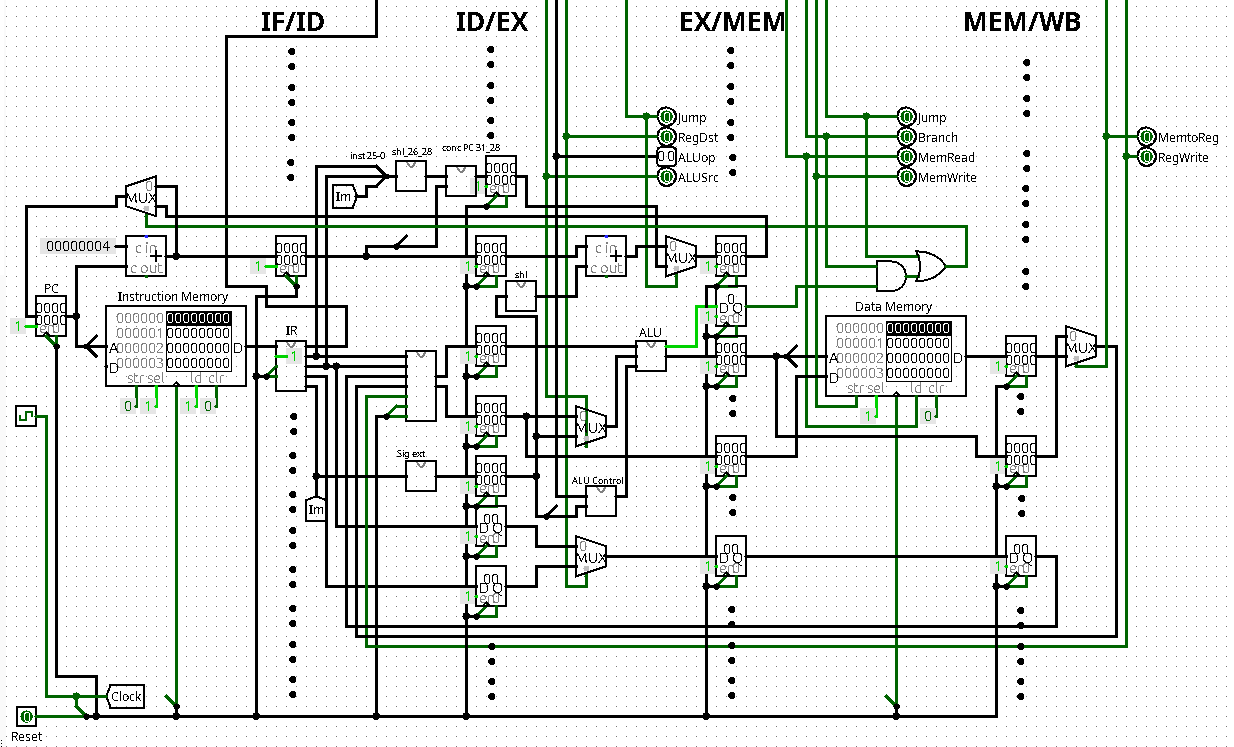
\includegraphics[width=\linewidth]{images/prints/Pipeline/Bloco Operativo Pipeline Antes.png}
            \caption{\label{print:pipeline_ob_before} MIPS Pipeline - Bloco Operativo Antes}
        \end{figure}

        Sobre essa versão do MIPS com pipeline, foram feitas as modificações listadas à seguir:
        \begin{itemize}
            \item Adicionada operação multiplicação na ALU;
            \item Adicionada saída dos bits superiores da multiplicação na ALU;
            \item Adicionada barreira temporal para capturar valor de RS;
            \item Adicionado MUX para o JR na entrada do PC;
            \item Corrigidos os timings entre barreiras temporais para o sinal de IsMult;
            \item Utilizado o sinal IsMult para não habilitar a escrita nos registradores;
            \item Propagado o sinal de imediato com 32 bits para a etapa de MEM;
            \item Colocado comparador de menor que 0 ou menor que RS para instruções de BLTZ e SLTIU em MEM;
            \item Conectado o BLTZ ao mux de branches;
            \item Propagado o bit de comparação RS < Imed para o estágio de MEM;
            \item Adicionado bit extender para o resultado da comparação acima;
            \item Conectado o resultado desse bit extender na entrada de escrita dos GPRs;
            \item Adicionado splitter para pegar os 8 bits menos significativos de um dado da memória;
            \item Extendido esses 8 bits acima;
            \item Conectado esse resultado controlado pelo sinal LB nos GPRs.
        \end{itemize}

        Com essas modificações listadas acima, obteve-se a seguinte nova representação do bloco operativo do MIPS:
        \begin{figure}[h!]
            \centering
            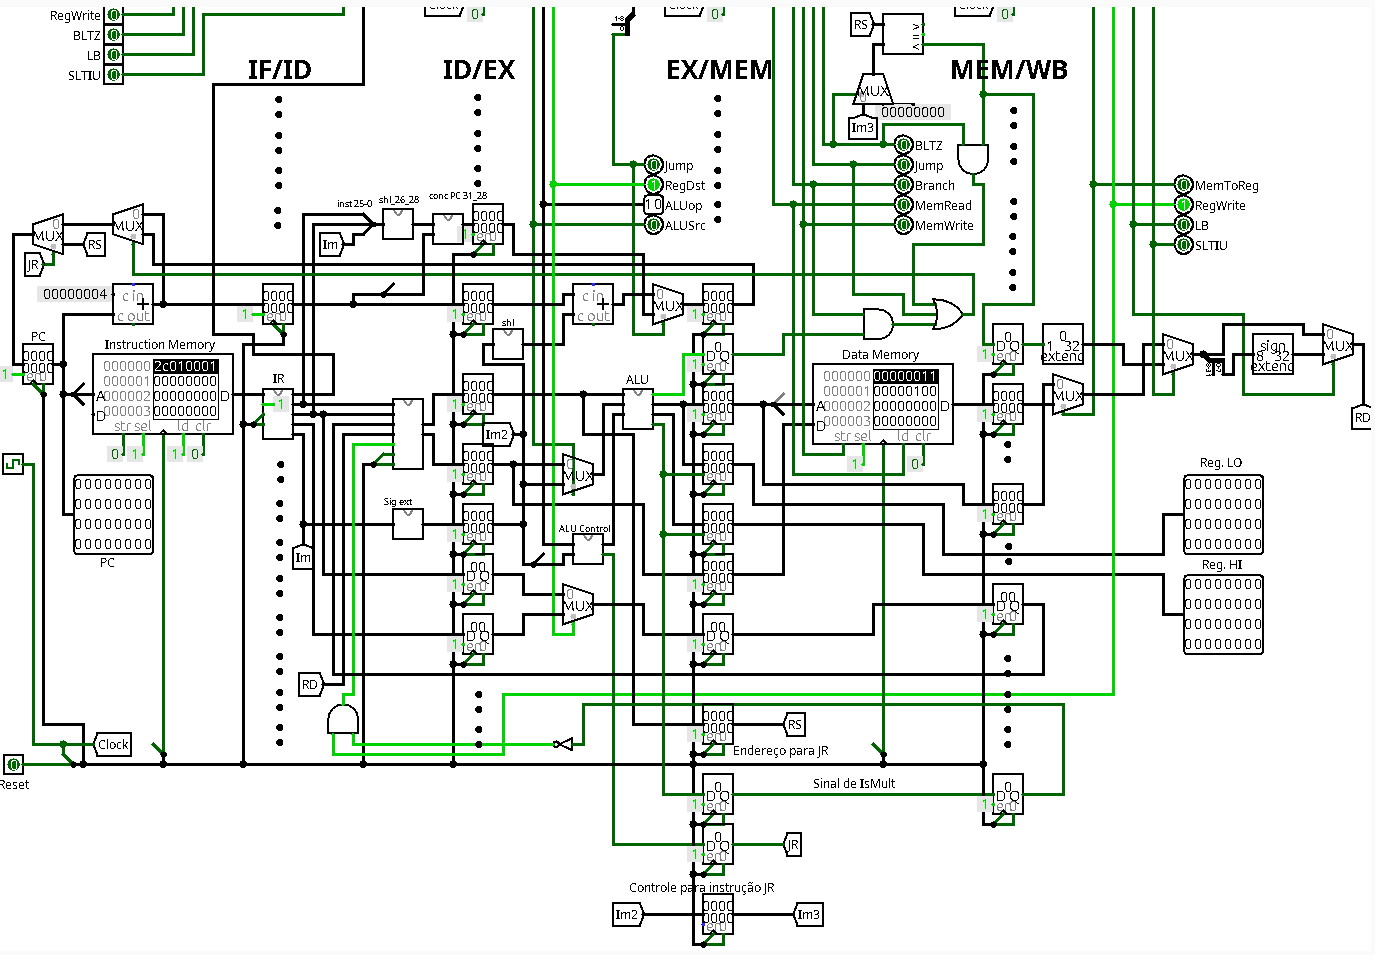
\includegraphics[width=\linewidth]{images/prints/Pipeline/Bloco Operativo Pipeline Depois.png}
            \caption{\label{print:pipeline_ob_after} MIPS Pipeline - Bloco Operativo Depois}
        \end{figure}

        \subsection{Modificações no Bloco de Controle}
        Já na parte de controle, anteriormente, tinha-se a seguinte representação:
        \begin{figure}[h!]
            \centering
            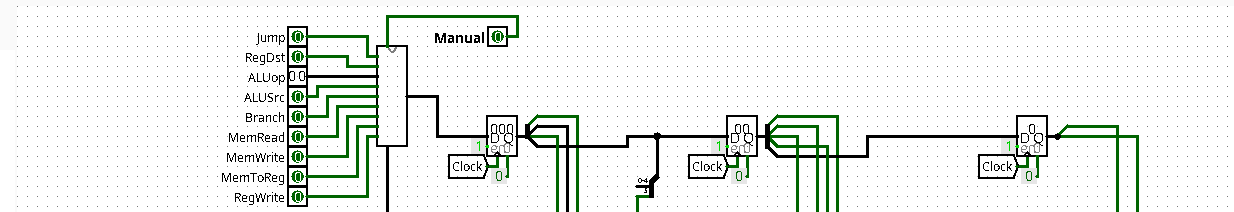
\includegraphics[width=\linewidth]{images/prints/Pipeline/Bloco de Controle Pipeline Antes.png}
            \caption{\label{print:pipeline_cb_before} MIPS Pipeline - Bloco Controle Antes}
        \end{figure}

        A partir dessa parte de controle, é possível listar as seguintes modificações:
        \begin{itemize}
            \item Criados os sinais de controle LB, SLTIU, BLTZ, JR e IsMult;
            \item Atualizado o ALU Control para as instruções de MULT e JR;
            \item Adicionada saída IsMULT da ALU;
            \item Adicionada barreira temporal para o estágio de EX/MEM do JR;
            \item Propagados todos os sinais de controle para as respectivas etapas do circuito:
                \subitem - BLTZ em MEM;
                \subitem - LB e SLTIU em WB.
        \end{itemize}

        Além dessas modificações, foram reordenados os sinais de controle para serem equivalentes aos sinais de controle do MIPS Singlecycle.
        Assim, as modificações da ROM de controle foram as mesmas listadas na seção do MIPS Singlecycle:
        \begin{itemize}
            \item ROM para JR: 0x0241 end 0x00;
            \item ROM para BLTZ: 0x0404 end 0x01;
            \item ROM para LB: 0x0B18 end 0x20;
            \item ROM para MULT: 0x0241 end 0x00;
            \item ROM para SLTIU: 0x1300 end 0x0B.
        \end{itemize}

        Com tudo isso, obteve-se o seguinte novo esquemático externo da parte de controle do MIPS com pipeline:
        \begin{figure}[h!]
            \centering
            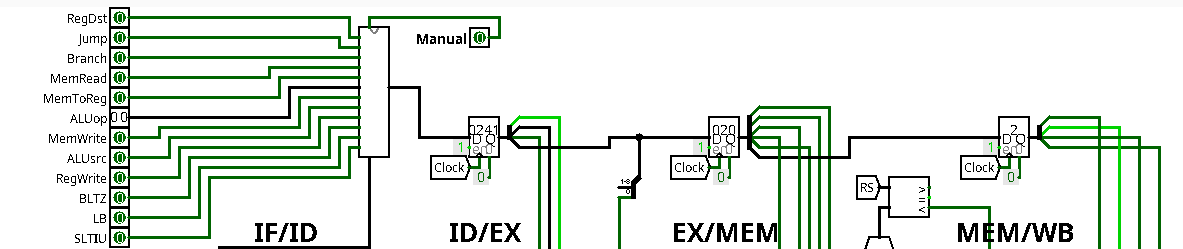
\includegraphics[width=\linewidth]{images/prints/Pipeline/Bloco de Controle Pipeline Depois.png}
            \caption{\label{print:pipeline_cb_after} MIPS Pipeline - Bloco Controle Depois}
        \end{figure}

        Algumas dessas modificações aqui listadas foram mostradas em mais detalhes na subseção anterior.

        \subsection{Testes de Implementação}
        Para comprovar que essas mudanças acima trouxeram a correta implementação das instruções especificados neste trabalho,
        abaixo seguem os testes realizados com imagens e a respectiva sequência de instruções:
        
        É importante notar, em todos os testes, que há uma grande quantidade de NOPs espalhados entre as instruções. Isso é devido
        a não terem sido implementadas soluções para lidar com dependências de dados e de controle.

        \begin{itemize}
            \item Teste da Instrução JR:
                \subitem 0x8C010000; LW: Reg1 $\leftarrow$ Mem[0] (64 ou 0x40)
                \subitem 0x00000000; NOP
                \subitem 0x00000000; NOP
                \subitem 0x00000000; NOP
                \subitem 0x00000000; NOP
                \subitem 0x00200008; JR: PC $\leftarrow$ Reg1 (64 ou 0x40)
        \end{itemize}
        
        \begin{figure}[h!]
            \centering
            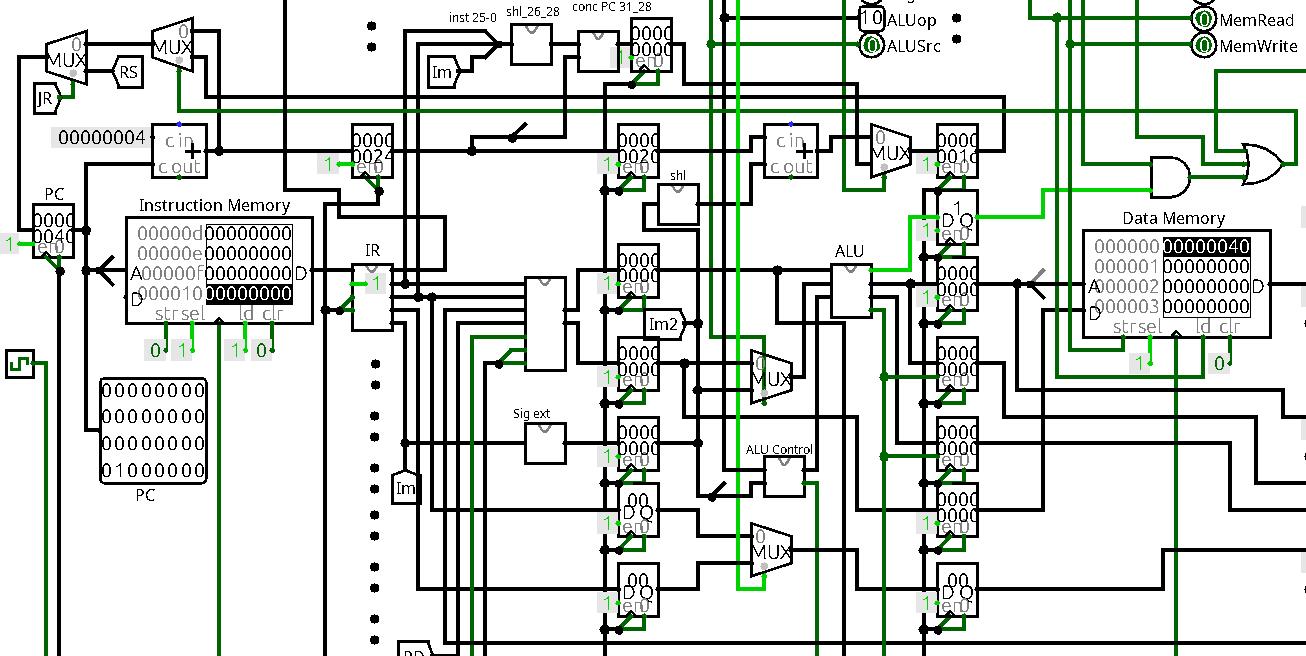
\includegraphics[width=\linewidth]{images/prints/Pipeline/Teste JR.png}
            \caption{\label{print:pipeline_test_JR} MIPS Pipeline - Teste JR}
        \end{figure}

        \begin{itemize}
            \item Teste da Instrução MULT:
                \subitem MULT: HI, LO $\leftarrow$ Reg1 $\cdot$ Reg2
                \subitem 0x8C010000; Reg1 $\leftarrow$ Mem[0] (17 ou 0x11)
                \subitem 0x8C020001; Reg2 $\leftarrow$ Mem[1] (256 ou 0x100)
                \subitem 0x00000000; NOP
                \subitem 0x00000000; NOP
                \subitem 0x00000000; NOP
                \subitem 0x00000000; NOP
                \subitem 0x00220018; HI, LO $\leftarrow$ Reg1 $\cdot$ Reg2 (HI = 0, LO = 4352 ou 0x10400)
        \end{itemize}
        
        \begin{figure}[h!]
            \centering
            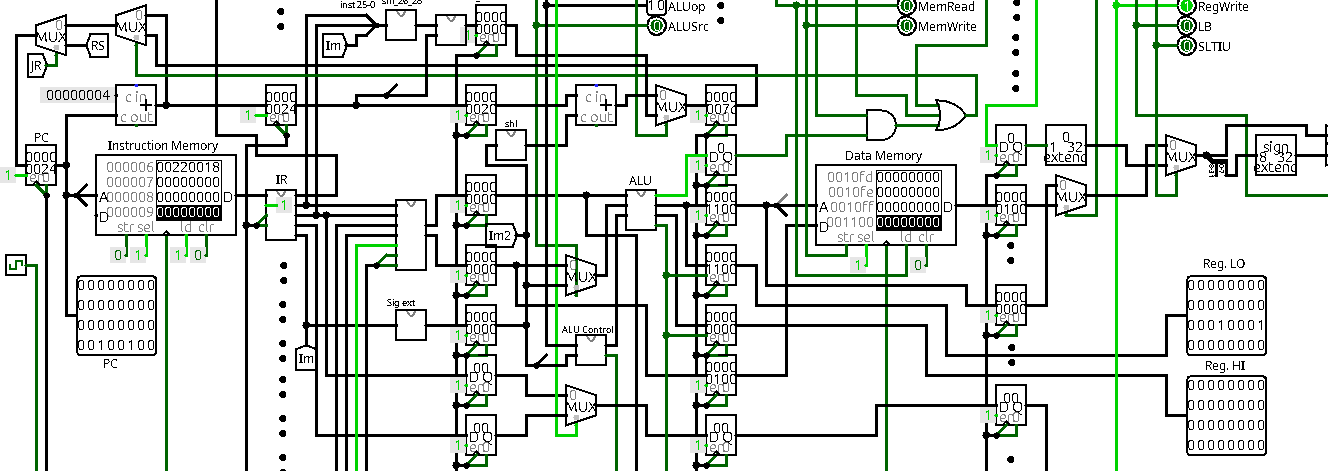
\includegraphics[width=\linewidth]{images/prints/Pipeline/Teste MULT.png}
            \caption{\label{print:pipeline_test_MULT} MIPS Pipeline - Teste MULT}
        \end{figure}

        \clearpage
        \begin{itemize}
            \item Teste da Instrução BLTZ:
                \subitem BLTZ: if Reg1 $<$ 0 then PC += IMED$\cdot$4 + 4 (IMED = 10)
                \subitem 0x8C010000; Reg1 $\leftarrow$ Mem[0] (-1 (0xFFFFFFFF))
                \subitem 0x00000000; NOP
                \subitem 0x00000000; NOP
                \subitem 0x00000000; NOP
                \subitem 0x00000000; NOP
                \subitem 0x0420000A; PC += IMED$\cdot$4 + 4 (PC = 64 ou 0x40)
        \end{itemize}
        
        \begin{figure}[h!]
            \centering
            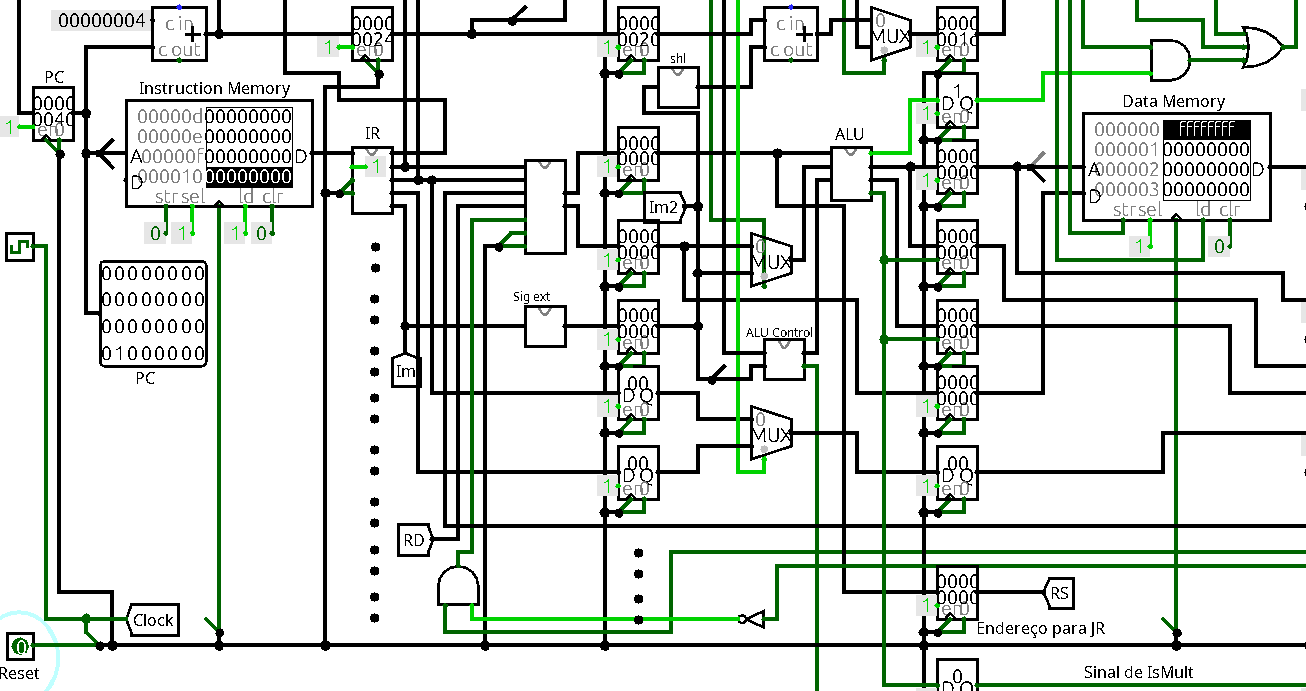
\includegraphics[width=\linewidth]{images/prints/Pipeline/Teste BLTZ.png}
            \caption{\label{print:pipeline_test_BLTZ} MIPS Pipeline - Teste BLTZ}
        \end{figure}

        \begin{itemize}
            \item Teste da Instrução LB:
                \subitem LB: Reg1 $\leftarrow$ byte(Mem[0]) (0x00000FFF)
                \subitem 0x80010000; Reg1 $\leftarrow$ byte(Mem[0]) (0xFFFFFFFF)
        \end{itemize}
        
        \begin{figure}[h!]
            \centering
            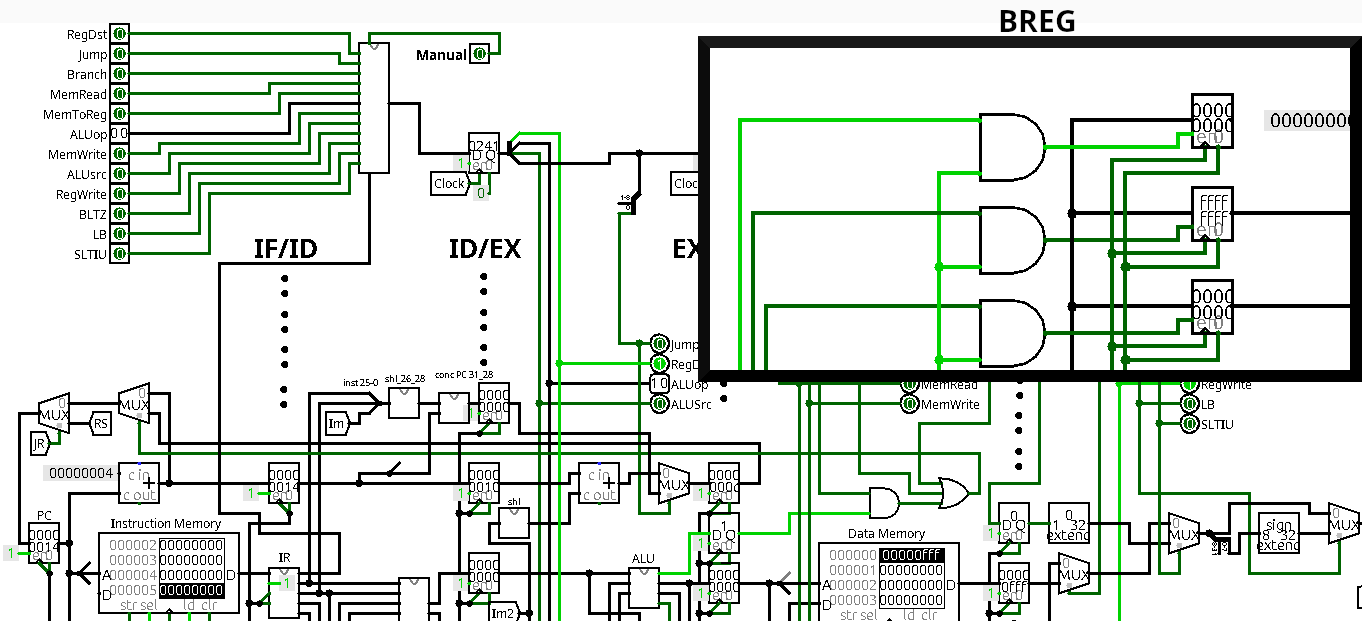
\includegraphics[width=\linewidth]{images/prints/Pipeline/Teste LB.png}
            \caption{\label{print:pipeline_test_LB} MIPS Pipeline - Teste LB}
        \end{figure}

        \clearpage
        \begin{itemize}
            \item Teste da Instrução SLTIU:
                \subitem SLTIU: Reg1 $\leftarrow$ Reg0 $<$ IMED (1)
                \subitem 0x2C010001; Reg1 $\leftarrow$ Reg0 $<$ 1 (Reg1 = 1)
        \end{itemize}
        
        \begin{figure}[h!]
            \centering
            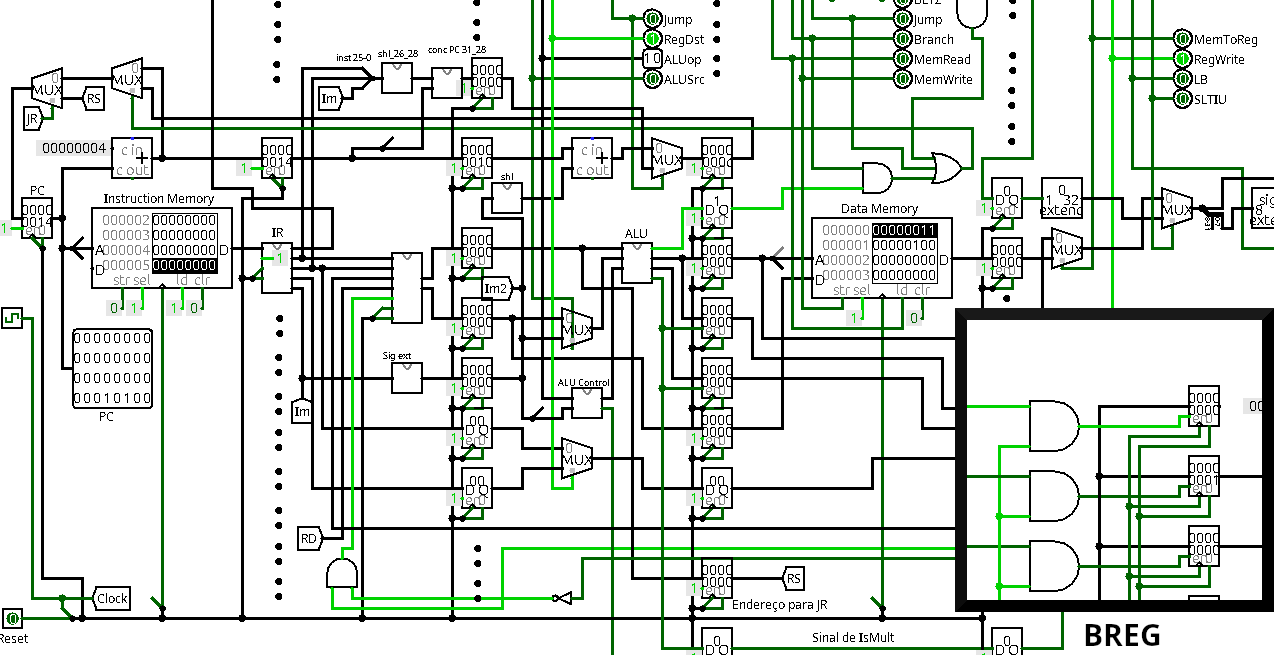
\includegraphics[width=\linewidth]{images/prints/Pipeline/Teste SLTIU.png}
            \caption{\label{print:pipeline_test_SLTIU} MIPS Pipeline - Teste SLTIU}
        \end{figure}

\end{document}
